
\subsection{Addition of Cobordisms}

We now make precise the notion of addition for $2$--dimensional thick tangles
mentioned in the previous subsection, so that non-elementary tensors become
accessible with parallel field theories.

Consider $2$--dimensional thick tangles $M : I^{\amalg n} \to I^{\amalg m}$ and
$N : I^{\amalg n'} \to I^{\amalg m'}$. Suppose $S_1 \in \set{S(M), S(N)}$ is the
source of either $M$ or $N$ with the most copies of $I$ and $S_0$ is that with
the least copies of $I$. $T_0, T_1 \in \set{T(M), T(N)}$ are defined
analogously. That is, $S_0 = I^{\amalg \min\set{m, m'}}$,
$T_0 = I^{\amalg \min\set{n, n'}}$, $S_1 = I^{\amalg \max\set{m, m'}}$ and
$T_1 = I^{\amalg \max\set{n, n'}}$. Then, $M + N$ is defined to be the shape
obtained by gluing $S_0$ to the first $\min\set{m, m'}$ copies of $I$ in
$S_1$ and $T_0$ to the first $\min\set{n, n'}$ copies of $I$ in $T_1$.

For instance, let $M$ be the pair-of-pants and $N$ the cylinder $I \times I$.
Then, pictorially, $M + N$ would look like\footnote{generated using
\cite{Mathcha}}:

\[
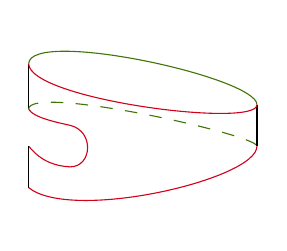
\begin{tikzpicture}[x=0.75pt,y=0.75pt,yscale=-1,xscale=1]
%Curve Lines [id:da6783491277813168]
\draw [color={rgb, 255:red, 208; green, 2; blue, 27 }  ,draw opacity=1 ]
(10,62.25) .. controls (12.6,66.54) and (25,68.8) .. (30,70) ;
%Curve Lines [id:da8932052500161816]
\draw [color={rgb, 255:red, 208; green, 2; blue, 27 }  ,draw opacity=1 ]
(10,80) .. controls (16.2,87.6) and (23,89.6) .. (30,90) ;
%Curve Lines [id:da5336367474763575]
\draw [color={rgb, 255:red, 208; green, 2; blue, 27 }  ,draw opacity=1 ]
(30,70) .. controls (41.8,72.8) and (40.6,90) .. (30,90) ;
%Straight Lines [id:da20283370527792666]
\draw (10,40.25) -- (10,62.25) ;
%Straight Lines [id:da4944370504980129]
\draw (10,80) -- (10,100) ;
%Curve Lines [id:da1547743895825433]
\draw [color={rgb, 255:red, 208; green, 2; blue, 27 }  ,draw opacity=1 ]
(10,100) .. controls (30.6,116.7) and (120.2,96) .. (120,80) ;
%Curve Lines [id:da9098653012878017]
\draw [color={rgb, 255:red, 65; green, 117; blue, 5 }  ,draw opacity=1 ]
(10,40.25) .. controls (11,23.2) and (119.8,46.8) .. (120,60) ;
%Curve Lines [id:da10875506317214012]
\draw [color={rgb, 255:red, 65; green, 117; blue, 5 }  ,draw opacity=1 ]
[dash pattern={on 4.5pt off 4.5pt}]  (10,62.25) .. controls (9.8,50) and
(119.8,74.4) .. (120,80) ;
%Straight Lines [id:da5956309013033436]
\draw    (120,60) -- (120,80) ;
%Curve Lines [id:da23301521900677968]
\draw [color={rgb, 255:red, 208; green, 2; blue, 27 }  ,draw opacity=1 ]
(10,40.25) .. controls (10.2,57.6) and (120.6,71.6) .. (120,60) ;
\end{tikzpicture}
\]
We note that this operation is distinct from both the disjoint union and the
gluing of thick tangles end-to-end. In particular, the results of this operation
can not, in general, be embeded into the infinite strip $\R \times I$. However,
we observe that we can unambiguously define the sources and targets of these
shapes as sources $S_1$ and $T_2$ respectively. We also observe that when
the domains and codomains of the summands are the same, the picture of a sum is
simply a diagram in $\DThick$ involving parallel cobordisms. This motivates us
to name these shapes as follows.

\begin{defn}
For thick tangles $M, N, S_0, T_0, S_1, T_1$ as above, $M + N$ is called a
multitangle $S_1 \to T_1$. In particular, we take the empty manifold to be
the empty sum -- a multitangle between any pair of objects in $\DThick$.
\end{defn}

\begin{rmk}
We observe that this definition carries over as is to transport graphs, bundles
and connections, even though the results of this kind of addition need not be
transport graphs, bundles or connections. In fact, if we take sums of three
cobordisms, then the result might even fail to be a manifold.
\TODO{Is it still a manifold?} Nevertheless, we will carry on with this
construction, being aware that we might start to lose some of the double
categorical structures.
\end{rmk}

However, we will observe that many of the useful structures in $\DThick$ are not
disturbed by this operation. We first define the starting data of yet another
double category:

\begin{enmrt}
\li Object category: same as $\TG\br{\CConn^V_{\DThick}}$
\li Morphism category: objects are sums of objects in
$\TG\br{\CConn^V_{\DThick}}$, including the empty sum, and morphisms are
piecewise isomorphisms -- that is, they are tuples of $2$--morphisms in
$\TG\br{\CConn^V_{\DThick}}$, one for each summand
\end{enmrt}

We would like to make our structure resemble an additive category. For this, we
will modify the definition of end-to-end gluing or horizontal composition so as
to make it bi-$\Z$--linear as follows. First, we will reduce diagrams involving
multibordisms into line diagrams of the following form, for simplicity:
\[\begin{tikzpicture}
\colvert{black}{1, 0}{s}
\colvert{black}{3, 0}{t}
\path
  (s) edge[bend left] (t)
  (s) edge (t)
  (s) edge[bend right] (t)
  ;
\end{tikzpicture}\]
where we shrink sources and targets to single vertices. Now, suppose that we
have thick tangles $M, M: X \to Y$ and $N, N' : Y \to Z$. Then, we can define
\[
  (N + N') * (M + M') := (N * M) + (M * M')
\]
since the relevant composites all exist. In line diagrams, this equation is:
\[\begin{tikzpicture}
\colvert{black}{1, 0}{X}
\colvert{black}{3, 0}{Y}
\lblvert{3.5, 0}{glue}{$\cdots$}
\colvert{black}{4, 0}{YY}
\colvert{black}{6, 0}{Z}
\path
  (X)  edge[bend left]   node[above]{$M$}   (Y)
  (X)  edge[bend right]  node[below]{$M'$}  (Y)
  (YY) edge[bend left]   node[above]{$N$}  (Z)
  (YY) edge[bend right]  node[below]{$N'$} (Z)
  ;
\lblvert{6.5, 0}{equals}{$:=$}
\colvert{black}{7, 0}{XX}
\colvert{black}{9, 0.30}{YYY}
\colvert{black}{9, -0.30}{YYYY}
\colvert{black}{11, 0}{ZZ}
\draw (XX) .. controls (7.5, 0.25) and (8.5, 0.30) .. (YYY);
\draw (YYY) .. controls (9.5, 0.30) and (10.5, 0.25) .. (ZZ);
\draw (XX) .. controls (7.5, -0.25) and (8.5, -0.30) .. (YYYY);
\draw (YYYY) .. controls (9.5, -0.30) and (10.5, -0.25) .. (ZZ);

\lblvert{9, 0.55}{NM}{$N * M$}
\lblvert{9, -0.55}{NNMM}{$N' * M'$}
\end{tikzpicture}\]
In other words, during horizontal composition of multitangles, we first undo
the gluing resulting from addition at the composition site and then perform the
gluing for horizontal composition.  This new gluing operation is easily seen to
be associative up to piecewise isomorphisms.
Furthermore, taking $M'$ to be the zero cobordism, we have
\[
  (N + N') * M = (N * M) + (N' * M)
\]
In pictures:
\[\begin{tikzpicture}
\colvert{black}{1, 0}{X}
\colvert{black}{3, 0}{Y}
\lblvert{3.5, 0}{glue}{$\cdots$}
\colvert{black}{4, 0}{YY}
\colvert{black}{6, 0}{Z}
\path
  (X)  edge   node[above]{$M$}   (Y)
  (YY) edge[bend left]   node[above]{$N$}  (Z)
  (YY) edge[bend right]  node[below]{$N'$} (Z)
  ;
\lblvert{6.5, 0}{equals}{$:=$}
\colvert{black}{7, 0}{XX}
\colvert{black}{9, 0.30}{YYY}
\colvert{black}{9, -0.30}{YYYY}
\colvert{black}{11, 0}{ZZ}
\draw (XX) .. controls (7.5, 0.25) and (8.5, 0.30) .. (YYY);
\draw (YYY) .. controls (9.5, 0.30) and (10.5, 0.25) .. (ZZ);
\draw (XX) .. controls (7.5, -0.25) and (8.5, -0.30) .. (YYYY);
\draw (YYYY) .. controls (9.5, -0.30) and (10.5, -0.25) .. (ZZ);

\lblvert{9, 0.55}{NM}{$N * M$}
\lblvert{9, -0.55}{NNMM}{$N' * M$}
\end{tikzpicture}\]
If, in addition, $M = Y \times I$, then we easily see that there is a piecewise
isomorphism $(N + N') * M \to N + N'$ -- that is, horizontal composition is
right unital up to isomorphism. Left unitality is similar -- let $M, M', N$ be
arbitrary and take $N'$ to be be zero. We should note that the addition of
(multi-)cobordisms does not have immediate objects but it is commutative up to
piecewise isomorphism. Hence, the morphism category of multitangles is an
up-to-isomorphism commutative monoid.

So far, we have defined addition on horizontal $1$--morphisms. We will define
addition on objects to fit this picture. Given $I^{\amalg m}$ and
$I^{\amalg m'}$, we define
\[
  I^{\amalg m} + I^{\amalg m'} := I^{\amalg \max\set{m, m'}}
\]
Without strictly verifying (or even defining) axioms further, we propose that
multitangles form a structure akin to an additive double category with
monoidal structure (given by disjoint union) -- in some loose sense, at the very
least. We invite the reader to formulate this notion of double category with
fully defined axioms to make our structure fit the definition.

We then move on to show that with this structure we have a more robust notion of
field theory capable of handling non-elementary tensors in the context of
quantum computing. To this end, we define:

\begin{defn}
We denote the ``additive monoidal double category'' of multitangles constructed
so far as $\TG^+(\CConn^V_{\DThick})$.
\end{defn}

